\documentclass[Ligatures=TeX,table,brazil,svgnames,usetotalslideindicator,comp
ress,10pt]{beamer}

\usetheme[titleformat=allsmallcaps]{metropolis}

\usepackage{polyglossia}
\setdefaultlanguage{brazil}
\disablehyphenation

\usepackage[cachedir=/tmp/minted-\jobname]{minted}
\usemintedstyle{pastie}

\usepackage{graphicx}
\graphicspath{{./figuras/}}

%\usepackage{textpos}

%\usepackage{xspace}
%\usepackage{mdwlist}
%\usepackage{siunitx}
\usepackage{alltt}
\usepackage{multicol}
\usepackage{multirow}
%\usepackage{amsmath}

\usepackage{cancel}
%\usepackage[simplified]{pgf-umlcd}
%\usepackage{pgf-umlsd}

\usepackage{smartdiagram}

\newcommand{\setcoverbg}{
    \setbeamertemplate{background}
     {
\includegraphics[width=\paperwidth,height=\paperheight]{backgrounds/coverbg}}
}
\newcommand{\setintersectionbg}{
    \setbeamertemplate{background}
     {
\includegraphics[width=\paperwidth,height=\paperheight]{backgrounds/blank}}
}
\newcommand{\setsectionbg}{
    \setbeamertemplate{background}
     {
\includegraphics[width=\paperwidth,height=\paperheight]{backgrounds/slidebg2}}
}


\title{Uma Brevíssima introdução à Java RMI}

\subtitle{MCTA025-13 - Sistemas Distribuídos}

\author{Emilio Francesquini e Fernando Teubl}
\institute{Centro de Matemática, Computação e Cognição\\ Universidade Federal do ABC}
\date{30 de junho de 2018}

\begin{document}

\setcoverbg
\maketitle

\setsectionbg

\begin{frame}
  \frametitle{Disclaimer}
  \begin{itemize}
  \item Estes slides foram preparados para o curso de \textbf{Sistemas
      Distribuídos na UFABC}.
  \item Este material pode ser usado livremente desde que sejam
    mantidos, além deste aviso, os créditos aos autores e
    instituições.
  \item Estes slides foram adaptados com base no material disponível
    em
    \begin{itemize}
      \item \url{https://docs.oracle.com/javase/tutorial/rmi/}
      \item \url{https://docs.oracle.com/javase/8/docs/platform/rmi/spec/rmiTOC.html}
      \item \url{https://www.tutorialspoint.com/java_rmi/index.htm}
    \end{itemize}
  \end{itemize}
\end{frame}

\begin{frame}
  \frametitle{Java RMI}
  \begin{itemize}
  \item Java \textbf{R}emote \textbf{M}ethod \textbf{I}nvocation
  \item Mecanismo que permite que JVMs (Java Virtual Machine)
    (\emph{i.e.} processos baseados em JVMs) possam se comunicar
    através da chamada de métodos remotos
  \item Facilita a comunicação entre os participantes de um
    sistema distribuído
  \item SDs criados com JRMI são tipicamente organizados como cliente/servidor mas nada
    impede que uma aplicação específica adote outras arquiteturas
  \item Aplicações distribuídas baseadas nesta tecnologia são
    frequentemente chamadas de \alert{sistemas de objetos
      distribuídos}.
  \end{itemize}
\end{frame}


\begin{frame}
  \frametitle{Arquitetura de uma aplicação RMI}
  \begin{figure}[ht]
    \centering
    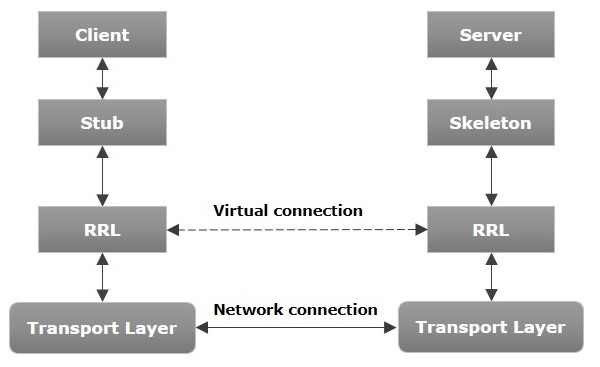
\includegraphics[width=\textwidth]{figuras/rmi_architecture.jpg}
    \\\tiny{Figura: \url{https://www.tutorialspoint.com/java_rmi}}
  \end{figure}
\end{frame}

\begin{frame}
  \frametitle{Arquitetura de uma aplicação RMI}
  \begin{itemize}
  \item \alert{Transport Layer} Esta camada faz a conexão entre o
    cliente e o servidor. Suas responsabilidades incluem criar, manter
    e descartar conexões.

  \item \alert{Stub} Um stub é uma representação (como objeto local)
    de um objeto remoto. Ele atua como um \emph{proxy} do objeto real
    na JVM do cliente para isto funcionando como intermediário na
    comunicação entre o programa cliente e o programa servidor.

  \item \alert{Skeleton} Localizado no servidor é o responsável por
    receber as requisições elaboradas pelos stubs dos clientes,
    repassá-las para o objeto apropriado e enviar a resposta (caso
    exista) para o cliente.

  \item \alert{RRL(Remote Reference Layer)} Esta camada se encarrega de controlar as referências aos objetos disponíveis remotamente para resolver, por exemplo, quando um objeto pode ser descartado pelo coletor de lixo.
  \end{itemize}
\end{frame}

\begin{frame}
  \frametitle{Funcionamento de uma aplicação RMI}
  \begin{itemize}
  \item Quando um \textbf{cliente faz uma chamada} para um método remoto ela é
    \textbf{tratada pelo Stub que a repassa para o RRL}
  \item Quando o \textbf{RRL-Cliente recebe a requisição do Stub} ele
    \textbf{entra em contato com o RRL-Servidor} (através da
    \emph{Transport Layer})
  \item Quando o \textbf{RRL-Servidor} recebe a requisição ele a \textbf{repassa ao
    Skeleton} que por sua vez faz a \textbf{requisição para o objeto remoto no
    servidor}.
  \item A \textbf{resposta}, caso exista, é então enviada seguindo-se o mesmo
    \textbf{caminho (reverso) até o cliente}.
  \end{itemize}
\end{frame}


\begin{frame}
  \frametitle{Empacotamento e Desempacotamento de Objetos}
  \begin{itemize}
  \item Quando uma chamada a um método de um objeto remoto que receba
    parâmetros é feita, é preciso fazer o \alert{empacotamento}
    (\emph{marshalling}) destes parâmetros para que sejam transmitidos
    pela rede até o servidor.
  \item O servidor, por sua vez, precisa fazer o
    \alert{desempacotamento} (\emph{unmarshalling}) desses parâmetros
    para repassá-los ao objeto.
  \item O mesmo processo é necessário para devolver ao cliente o
    resultado da chamada do método caso ele devolva um valor.
  \item Podem ser empacotados/desempacotados: tipos primitivos e
    objetos que implementem a interface \texttt{java.io.Serializable}
  \end{itemize}
\end{frame}

\begin{frame}
  \frametitle{Localizando Objetos Remotos - RMI Registry}
  \begin{itemize}
  \item O \alert{RMI Registry} mantém um catálogo com os
    objetos remotos colocados a disposição
  \item Toda vez que um processo deseja colocar um objeto a disposição
    dos clientes ele o \alert{registra} (\emph{bind}) no RMI Registry
  \item Quando um cliente deseja encontrar um objeto remoto ele
    \alert{consulta} (\emph{lookup}) o RMI Registry para obter uma
    referência àquele objeto (representada pelo stub)
  \end{itemize}
\end{frame}

\begin{frame}
  \frametitle{RMI Registry}
  \begin{figure}[ht]
    \centering
    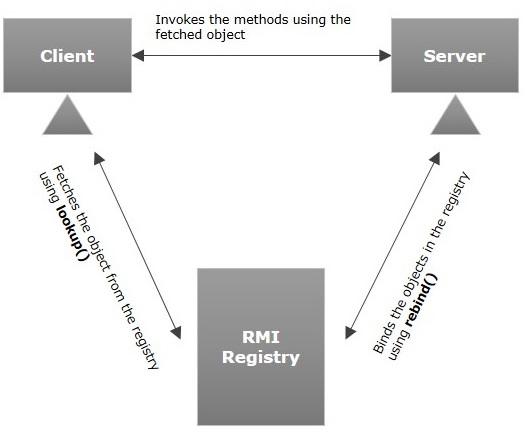
\includegraphics[width=0.8\textwidth]{figuras/registry.jpg}
    \\\tiny{Figura: \url{https://www.tutorialspoint.com/java_rmi}}
  \end{figure}
\end{frame}

\begin{frame}
  \frametitle{Desenvolvendo uma aplicação com RMI}
  \begin{itemize}
  \item Como qualquer outra aplicação em Java, uma aplicação com RMI é
    baseada em classes e interfaces
    \begin{itemize}
    \item Interfaces declaram métodos, classes implementam métodos
    \end{itemize}
  \item Objetos cujos métodos podem ser chamados entre JVMs distintas
    são chamados objetos remotos.
  \item Numa aplicação distribuída alguns objetos da aplicação podem
    ser \alert{locais} e outros \alert{remotos}.
  \item \textbf{Para se tornar um objeto remoto um objeto} \alert{precisa} implementar
    uma interface remota
    \begin{itemize}
    \item Uma interface remota estende a interface \texttt{java.rmi.Remote}
    \item Todos os métodos de uma interface remota devem lançar a
      exceção \texttt{java.rmi.RemoteException}
    \end{itemize}
  \end{itemize}
\end{frame}

\begin{frame}
  \frametitle{Desenvolvendo uma aplicação RMI}
  Os passos básicos abaixo descrevem o que é preciso ser feito para criar uma aplicação RMI
  \begin{itemize}
  \item Definir as interfaces remotas da aplicação
    \begin{itemize}
    \item Quais são objetos e os métodos relevantes para a aplicação
    \end{itemize}
  \item Desenvolver a classe contendo a implemtação do objeto
    \begin{itemize}
    \item É comum pelo menos parte do sistema que deseja-se tornar
      distribuído já existir, neste caso se faz necessário adaptá-lo
      para ficar compatível com a interface remota definida no passo
      anterior
    \end{itemize}
  \item Desenvolver o servidor
  \item Desenvolver o cliente
  \end{itemize}

\end{frame}

\begin{frame}
  \frametitle{Visão geral}
  \begin{figure}[ht]
    \centering
    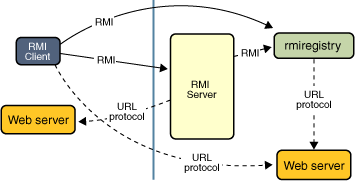
\includegraphics[width=0.8\textwidth]{figuras/rmi-2.png}
    \\\tiny{Figura: \url{https://docs.oracle.com/javase/tutorial/rmi/}}
  \end{figure}

\end{frame}


\begin{frame}
  \frametitle{Exemplo: Calculadora Simples}
  \begin{itemize}
  \item Como exemplo vamos desenvolver uma calculadora simples, que
    aceita as 4 operações aritméticas básicas
  \item Apesar de não ser necessário, por motivos didáticos vamos
    fazer com que os parâmetros não sejam tipos primitivos
    (\texttt{int,float,double}) mas um tipo \texttt{Numero} que vamos
    criar
  \end{itemize}

\end{frame}

\begin{frame}
  \frametitle{A Interface Número}
  \inputminted[linenos]{java}{Codigo/Aula02/Numero.java}
\end{frame}

\begin{frame}
  \frametitle{A Classe Número}
  \inputminted[linenos]{java}{Codigo/Aula02/NumeroImpl.java}
\end{frame}

\begin{frame}
  \frametitle{A Interface Calculadora}
  \inputminted[linenos]{java}{Codigo/Aula02/Calculadora.java}
\end{frame}

\begin{frame}
  \frametitle{A Classe Calculadora}
  {\footnotesize
    \inputminted[linenos]{java}{Codigo/Aula02/CalculadoraImpl.java}
    }
\end{frame}

\begin{frame}
  \frametitle{O Servidor}
  {\footnotesize
    \inputminted[linenos]{java}{Codigo/Aula02/ServidorCalculadora.java}
    }
\end{frame}

\begin{frame}
  \frametitle{O Cliente - Parte 1}
  {\footnotesize
    \inputminted[linenos, firstline=1,
    lastline=14]{java}{Codigo/Aula02/ClienteCalculadora.java}
  }
\end{frame}

\begin{frame}
  \frametitle{O Cliente - Parte 2}
  {\footnotesize
    \inputminted[linenos, firstline=16,
    lastline=27]{java}{Codigo/Aula02/ClienteCalculadora.java}
  }
\end{frame}

\begin{frame}
  \frametitle{O Cliente - Parte 3}
  {\footnotesize
    \inputminted[linenos, firstline=29]
    {java}{Codigo/Aula02/ClienteCalculadora.java}
  }
\end{frame}

\begin{frame}[fragile]
  \frametitle{Executando a aplicação - RMI Registry}

  É preciso iniciar o \emph{registry} e então o servidor para que ele
  registre a calculadora.

\begin{minted}{bash}
$ rmiregistry

\end{minted}

Não é dada nenhuma saída, a menos que outro registry já esteja em execução. Neste caso:
{\footnotesize
\begin{minted}{bash}
$ rmiregistry
java.rmi.server.ExportException: Port already in use: 1099; nested exception is:
        java.net.BindException: Address already in use (Bind failed)
        ...
\end{minted}
}
\end{frame}

\begin{frame}[fragile]
  \frametitle{Executando a aplicação}

  Em um outro terminal, inicie o servidor:

\begin{minted}{bash}
$ java ServidorCalculadora
Servidor iniciado.

\end{minted}

E finalmente o cliente:

\begin{minted}{bash}
$ java ClienteCalculadora
Resultados obtidos do servidor:
        +:7.0
        -:-1.0
        *:12.0
        /:0.75
Tentou dividir por zero! Esta é uma exceção remota.
$
\end{minted}

\end{frame}

\begin{frame}
  \frametitle{Exercício}

  Implemente um servidor de chat com suporte a múltiplos clientes (a
  exemplo do que foi feito na Aula 1) utilizando JRMI.

\end{frame}

\end{document}